\chapter{Diseño Dinámico e Interacción Técnica (PlantUML)}

\section{Estándar de Modelado Dinámico en PlantUML}
A diferencia de los diagramas conceptuales abstractos, los diagramas de secuencia de \textbf{SYSELL Web v2.0} fueron codificados en \textbf{PlantUML} bajo la directiva \texttt{skinparam style strictuml}. Cada diagrama modela con exactitud los mensajes síncronos y asíncronos que atraviesan las cuatro capas de la arquitectura del software:
\begin{enumerate}
    \item \textbf{Capa de Presentación (UI / SPA):} Cliente web interactivo en React 18 / TypeScript.
    \item \textbf{Capa de Controladores API:} Endpoints RESTful en Laravel que aplican validaciones de formulario, sanitización y middlewares de autorización.
    \item \textbf{Capa de Aplicación (Application Service):} Handlers de Commands y Queries que orquestan las reglas de negocio desacopladas.
    \item \textbf{Capa de Dominio y Persistencia:} Entidades de negocio y Repositorios que interactúan con MySQL 8.0 bajo transacciones ACID.
\end{enumerate}

\section{Catálogo de los 8 Diagramas de Secuencia Técnicos}
Se diseñaron 8 diagramas de secuencia que cubren la totalidad de los flujos críticos del sistema:

\begin{table}[H]
\centering
\small
\begin{tabularx}{\textwidth}{>{\ttfamily\centering}p{1.4cm} >{\raggedright\bfseries}p{4cm} >{\ttfamily\centering}p{1.8cm} Y}
\toprule
\textbf{Código} & \textbf{Diagrama de Secuencia} & \textbf{Caso de Uso} & \textbf{Lógica Técnica Modelada} \\
\midrule
DS-01 & Autenticación JWT y Bloqueo & CU-01 & Verificación Bcrypt, generación de token y bloqueo automático al 3er fallo consecutivo. \\
\addlinespace
DS-02 & Registro de Prendas y Catálogos & CU-05, CU-07 & Validación de atributos en catálogos cerrados, cálculo de SKU único y persistencia. \\
\addlinespace
DS-03 & Transacción de Venta POS & CU-08, CU-09 & Validación de stock, liquidación con pagos mixtos, descuento atómico y ticket digital. \\
\addlinespace
DS-04 & Ajuste de Stock en Kardex & CU-06 & Asiento manual por el Administrador con justificación obligatoria y recálculo de saldo. \\
\addlinespace
DS-05 & Reporte y Exportación de Ventas & CU-13, CU-14 & Consultas agregadas con filtros multicriterio y compilación en PDF/Excel. \\
\addlinespace
DS-06 & Gestión y Desbloqueo de Usuarios & CU-02 & CRUD de colaboradores, cambio de local, reseteo de clave y reinicio de intentos a 0. \\
\addlinespace
DS-07 & Catálogo Digital Web Público & CU-15 & Consulta pública sin autenticación, filtros AND y stock referencial por tienda física. \\
\addlinespace
DS-08 & Anulación de Venta Comercial & CU-12 & Validación de clave de Admin, cambio de estado y restitución atómica de existencias. \\
\bottomrule
\end{tabularx}
\caption{Suite de Diagramas de Secuencia Técnicos formalizados en SYSELL Web}
\label{tab:diagramas_secuencia}
\end{table}

\section{Análisis de Flujos Transaccionales Críticos con Evidencia Gráfica}

\subsection{Autenticación y Bloqueo Preventivo (DS-01)}
El flujo modela la recepción del payload JSON con credenciales en \texttt{/api/auth/login}. El servicio recupera el usuario por su \texttt{username}; si la cuenta no está bloqueada ni inactiva, compara la clave recibida mediante \texttt{password\_verify()} con el hash almacenado. Si la verificación falla:
\begin{lstlisting}[language=SQL]
UPDATE usuarios 
SET intentos_fallidos = intentos_fallidos + 1,
    bloqueado = CASE WHEN intentos_fallidos + 1 >= 3 THEN 1 ELSE 0 END
WHERE id = ?;
\end{lstlisting}
Si el contador alcanza 3, el estado pasa de inmediato a \texttt{bloqueado = 1}, denegando futuras peticiones y registrando el evento en la bitácora de auditoría.

\begin{figure}[H]
\centering
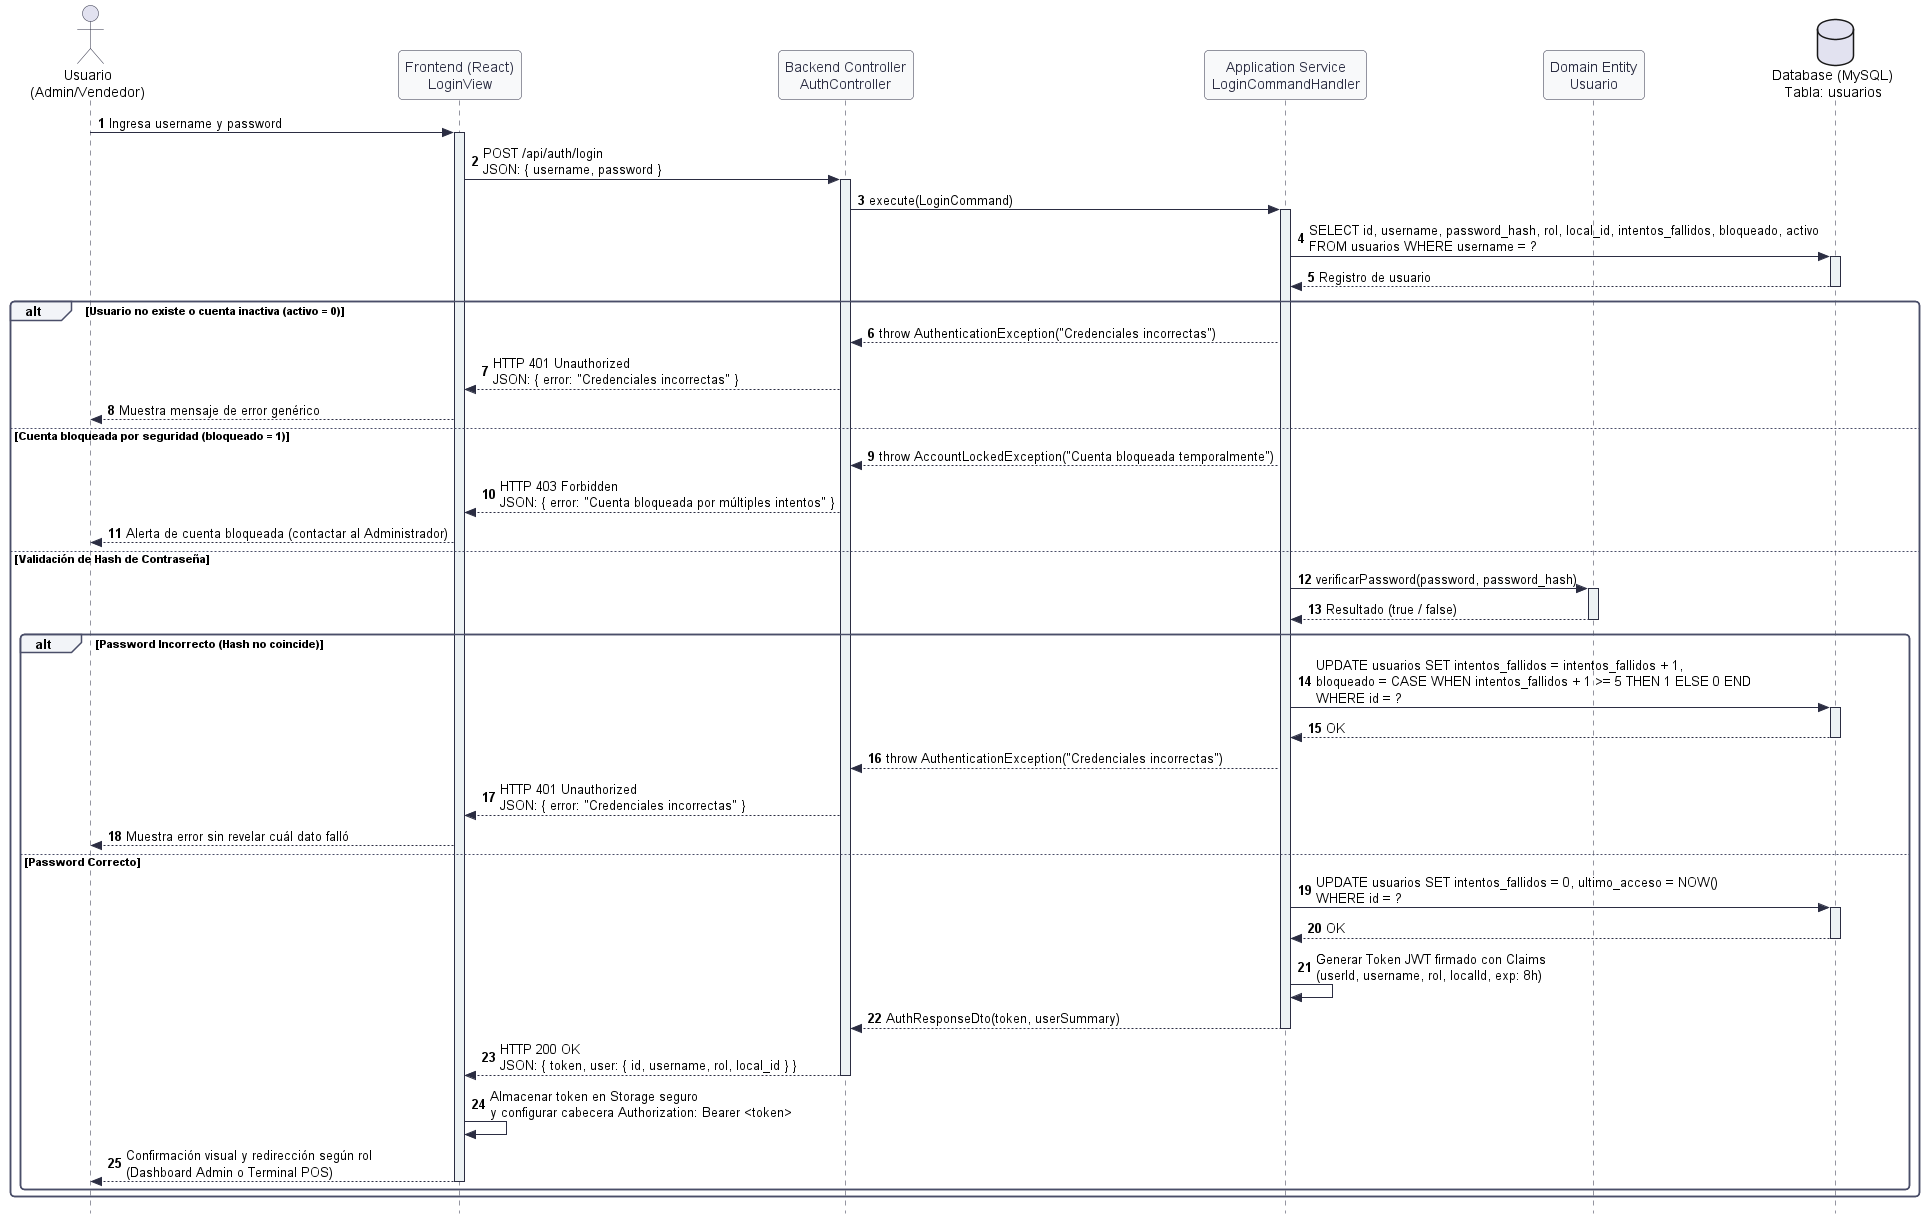
\includegraphics[width=0.92\textwidth]{ds_01_autenticacion_jwt.png}
\caption{Diagrama de Secuencia DS-01: Autenticación JWT y Bloqueo al 3er Intento}
\label{fig:ds_01}
\end{figure}

\subsection{Registro de Prendas y Desglose de Variantes (DS-02)}
El administrador registra una prenda base vinculándola a catálogos cerrados. El sistema genera de forma cartesiana las variantes de talla y color asignando los códigos SKU normalizados:

\begin{figure}[H]
\centering
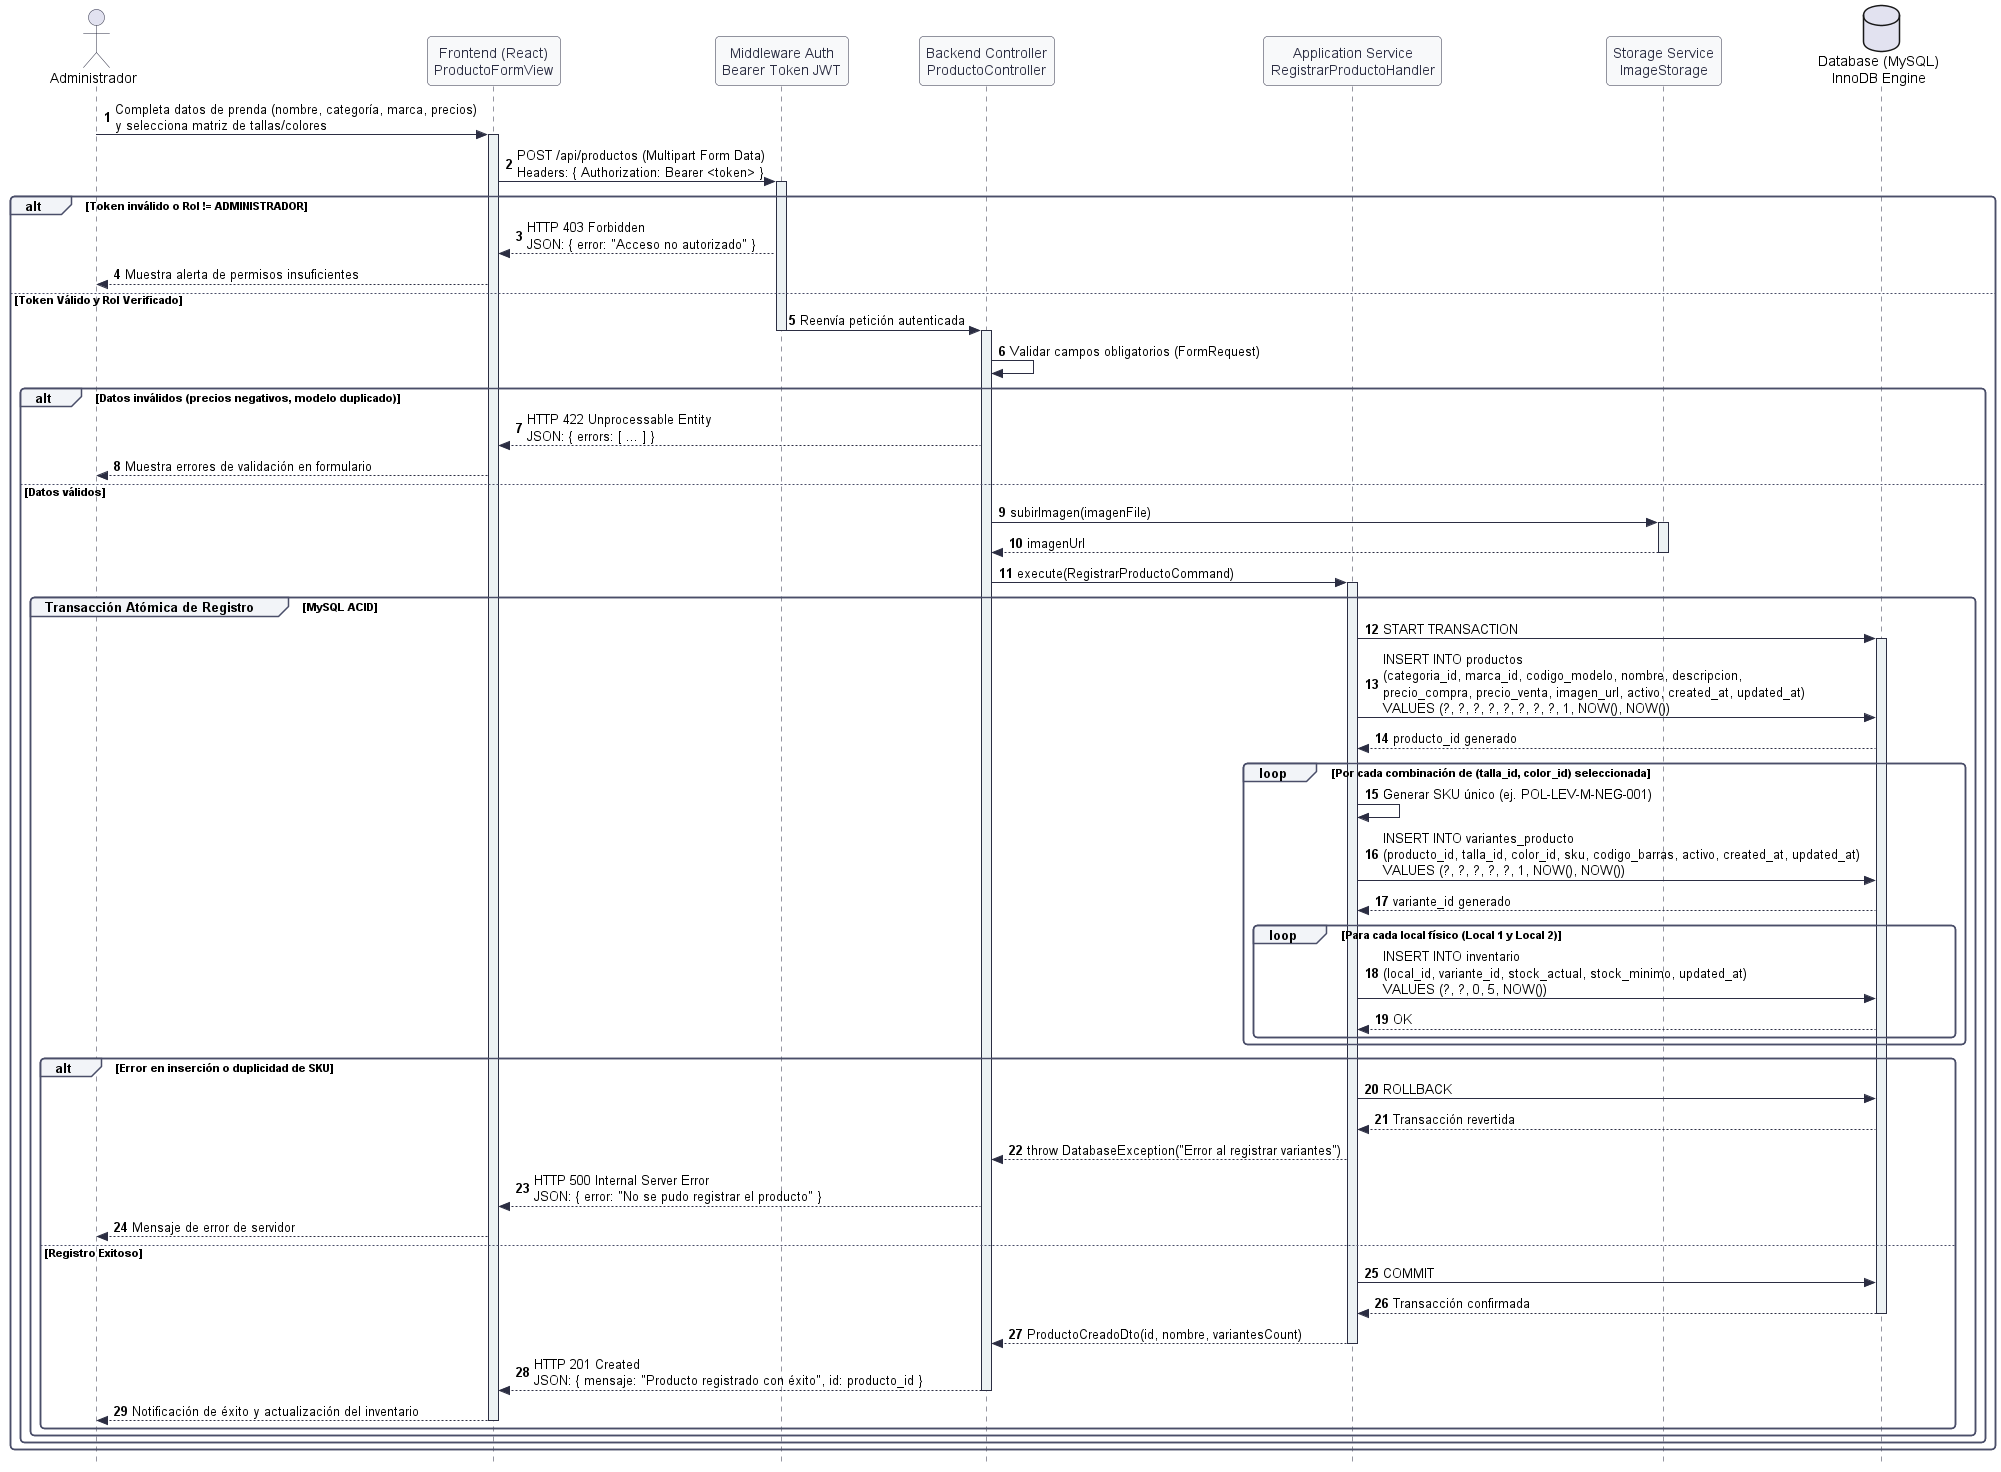
\includegraphics[width=0.92\textwidth]{ds_02_registro_producto_variantes.png}
\caption{Diagrama de Secuencia DS-02: Registro de Prenda Base y Variantes por SKU}
\label{fig:ds_02}
\end{figure}

\subsection{Transacción Atómica de Venta POS (DS-03)}
Para evitar inconsistencias en el inventario ante concurrencia o caídas de red, el proceso de confirmación de venta se ejecuta dentro de una transacción ACID (\textit{Database Transaction}):
\begin{enumerate}
    \item Inicio de transacción (\texttt{START TRANSACTION}).
    \item Inserción del encabezado en \texttt{ventas} con numeración correlativa única (\texttt{numero\_ticket}).
    \item Inserción de las líneas en \texttt{detalle\_ventas}.
    \item Descuento de stock en la tabla \texttt{inventario} para el local emisor:
    \begin{lstlisting}[language=SQL]
    UPDATE inventario 
    SET stock_actual = stock_actual - ? 
    WHERE local_id = ? AND variante_id = ? AND stock_actual >= ?;
    \end{lstlisting}
    \item Inserción de los medios de pago aplicados en \texttt{pagos\_venta}.
    \item Confirmación definitiva (\texttt{COMMIT}). En caso de cualquier falla de validación o stock insuficiente, se aborta la operación completa (\texttt{ROLLBACK}).
\end{enumerate}

\begin{figure}[H]
\centering
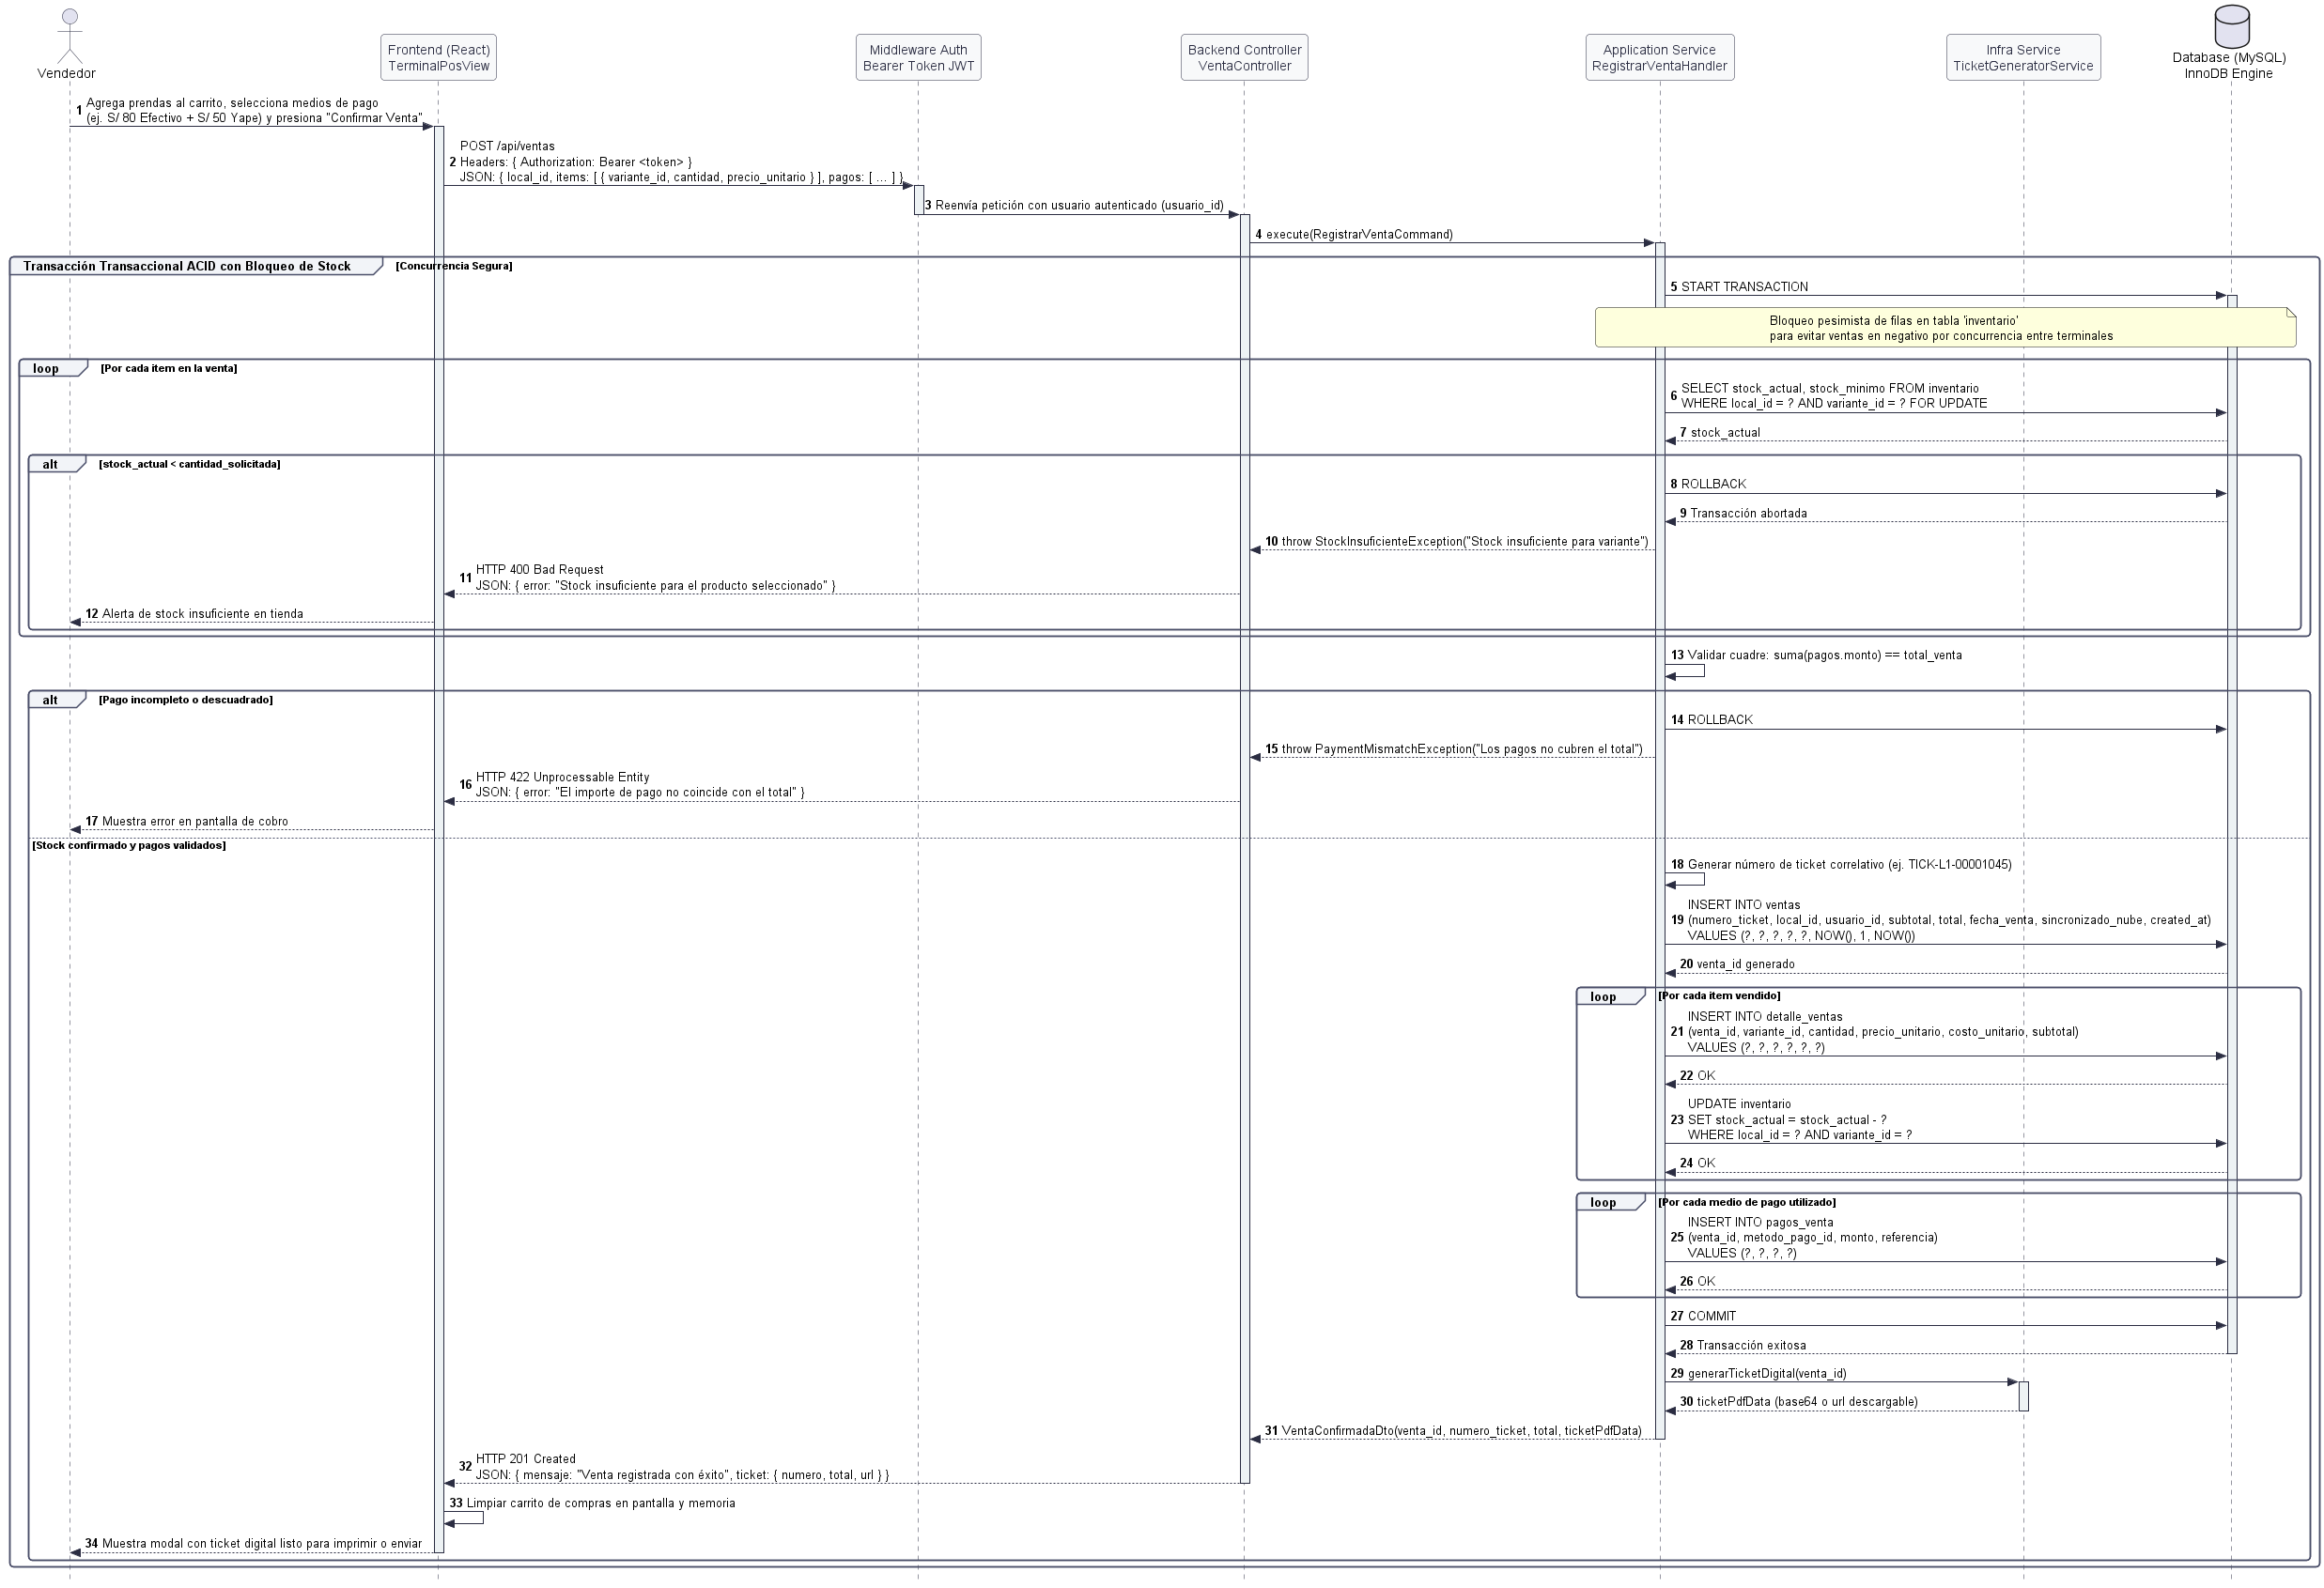
\includegraphics[width=0.92\textwidth]{ds_03_transaccion_venta_pos.png}
\caption{Diagrama de Secuencia DS-03: Transacción Atómica de Venta en Terminal POS}
\label{fig:ds_03}
\end{figure}

\subsection{Ajuste Manual de Existencias en Kardex (DS-04)}
Cualquier modificación manual del inventario físico requiere autorización del administrador, motivo explícito y registro de saldo previo y posterior:

\begin{figure}[H]
\centering
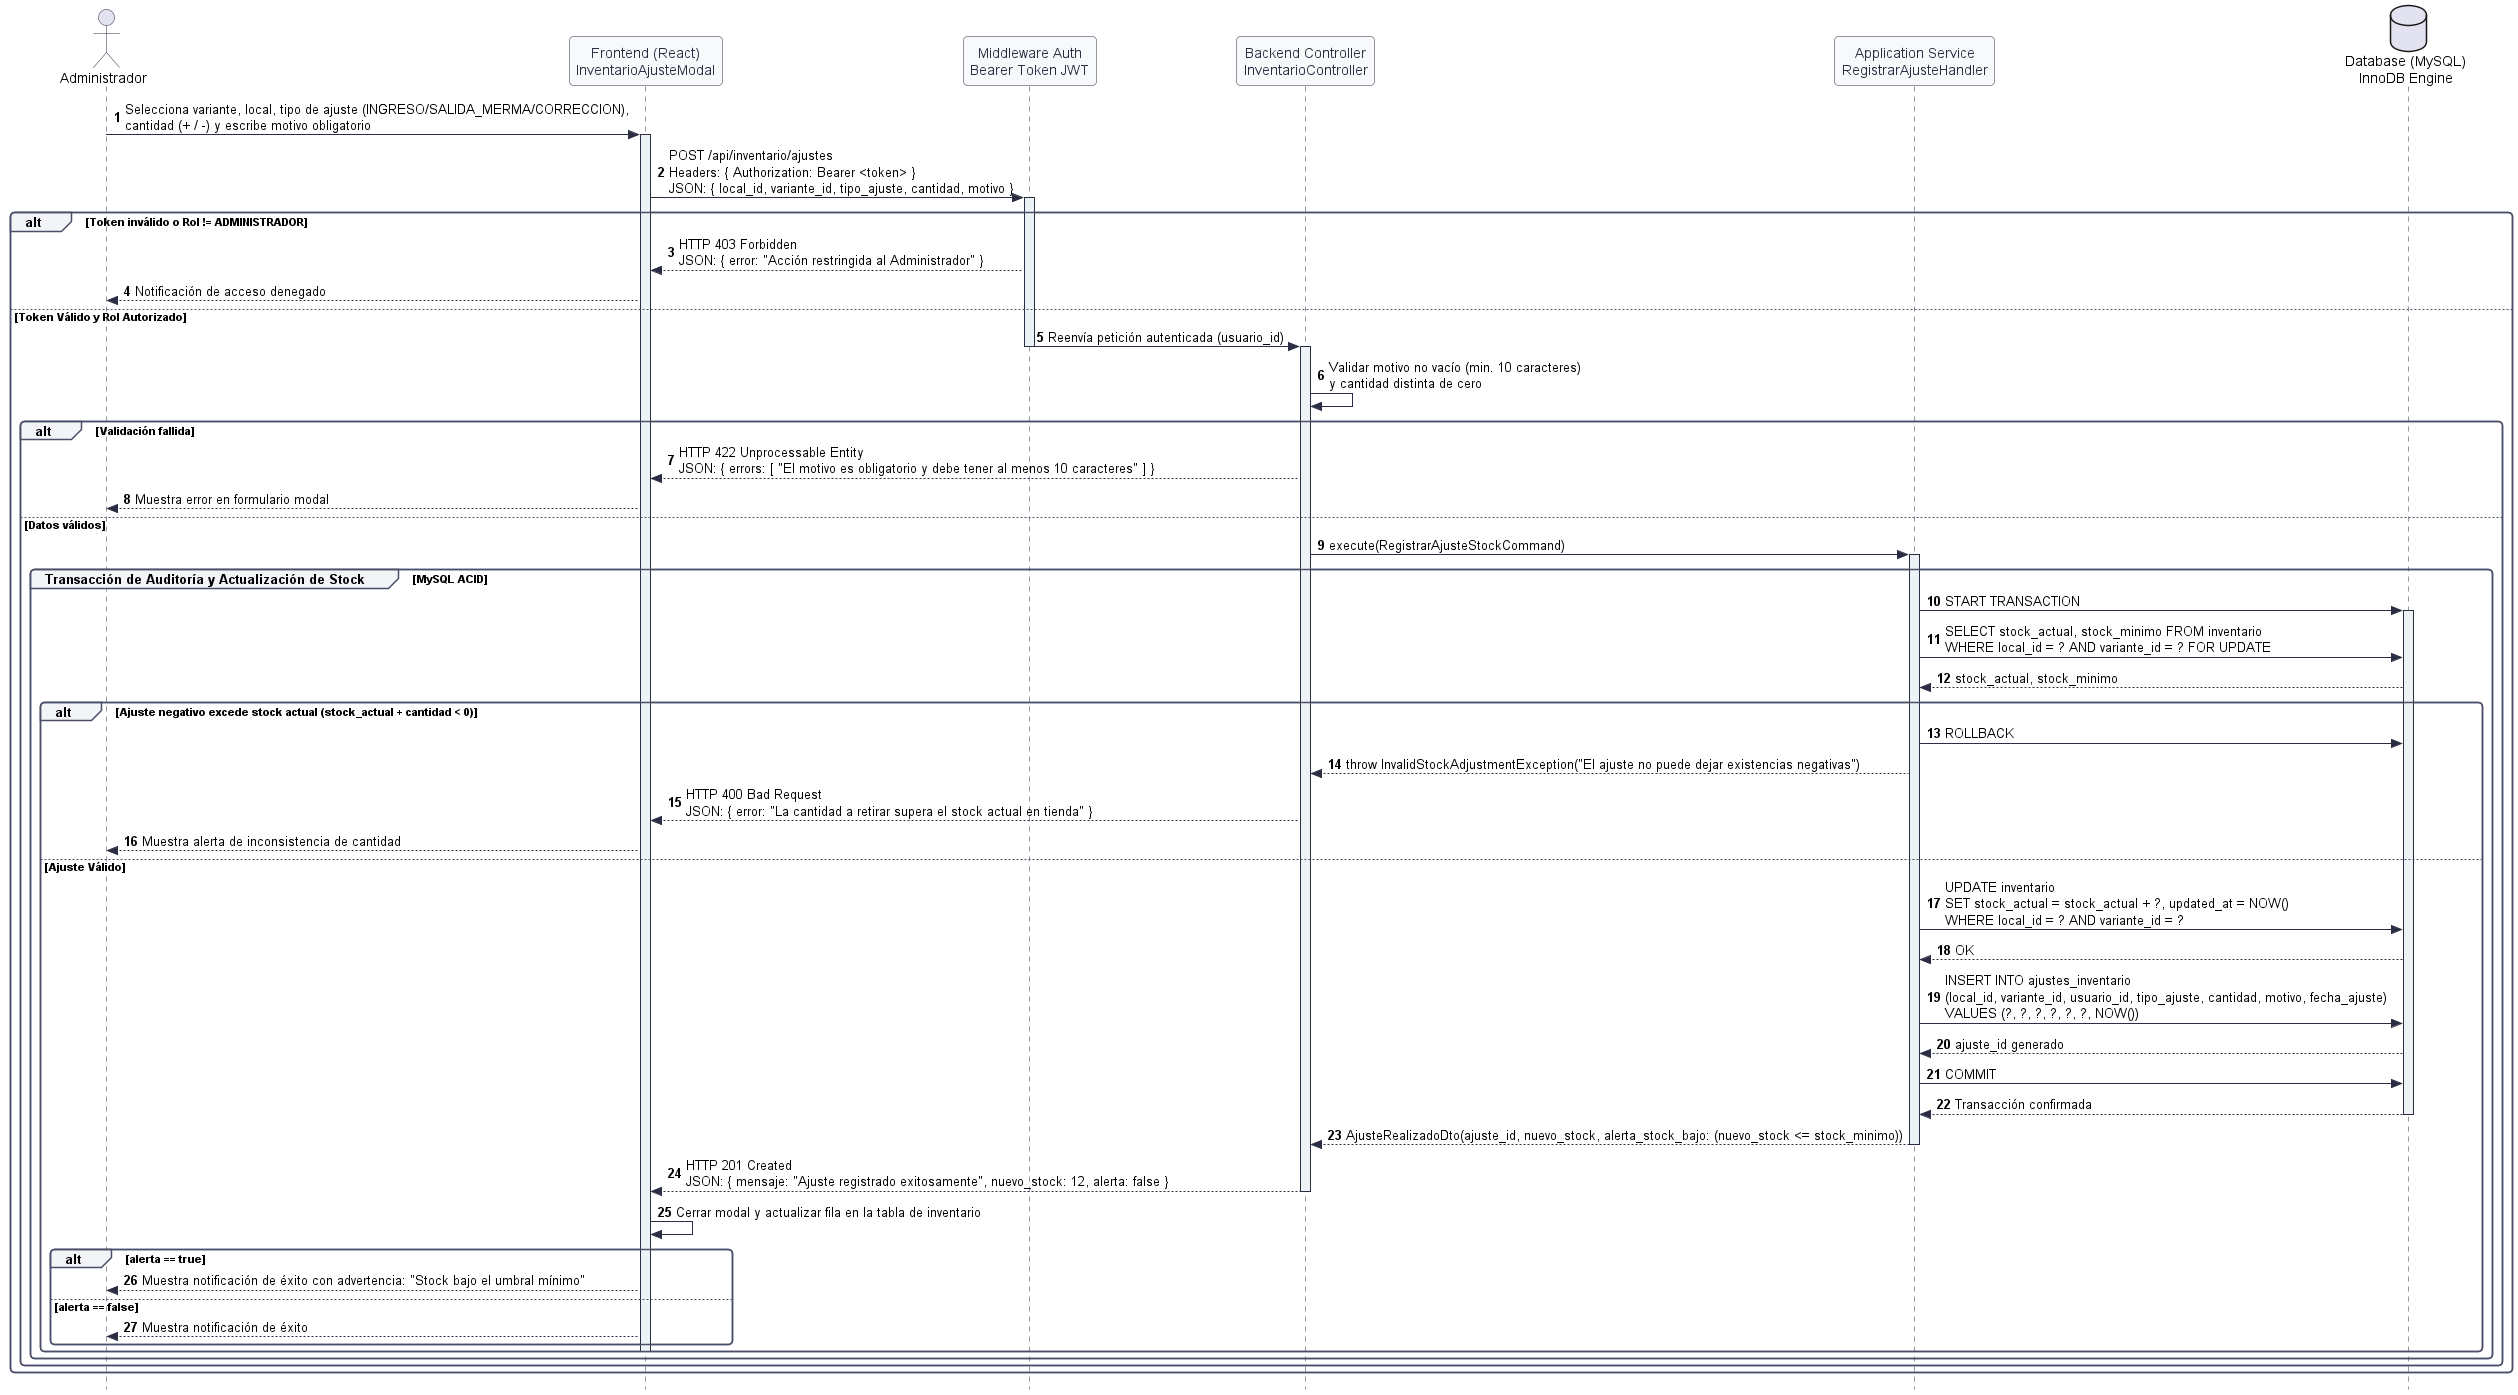
\includegraphics[width=0.92\textwidth]{ds_04_ajuste_inventario_kardex.png}
\caption{Diagrama de Secuencia DS-04: Ajuste de Inventario Físico y Movimiento de Kardex}
\label{fig:ds_04}
\end{figure}

\subsection{Generación y Exportación de Reportes Gerenciales (DS-05)}
Las consultas analíticas leen vistas optimizadas agregando ventas por sucursal, vendedor y rotación sin bloquear las tablas de caja:

\begin{figure}[H]
\centering
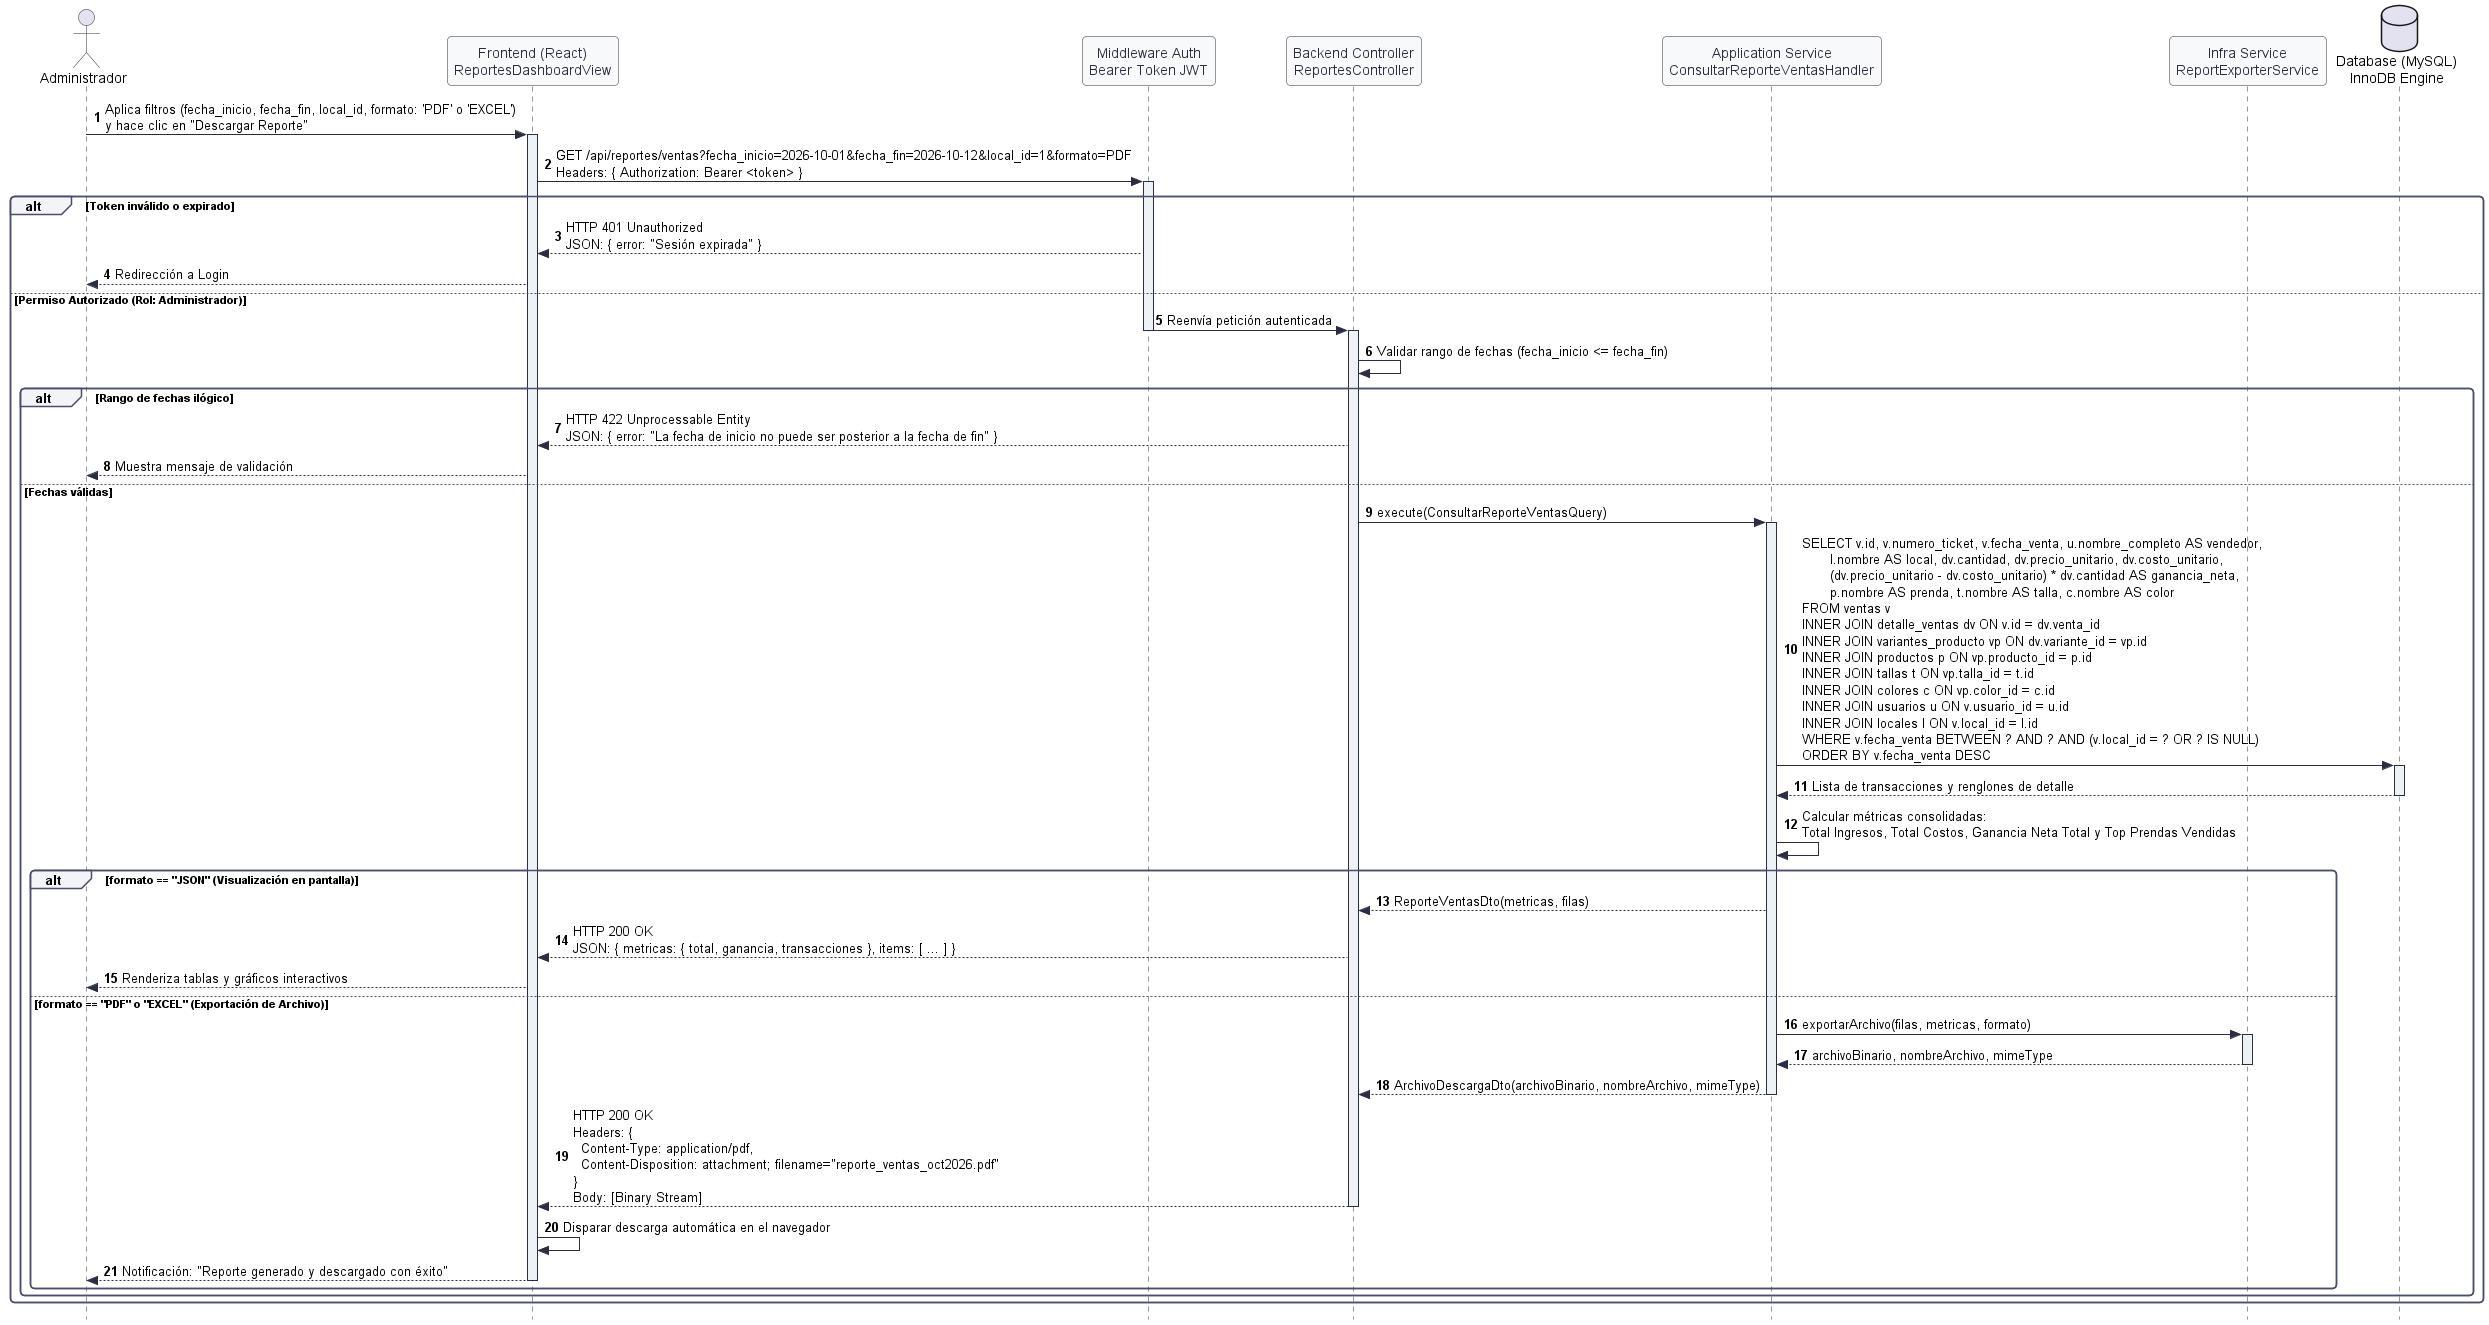
\includegraphics[width=0.92\textwidth]{ds_05_generacion_reporte_ventas.png}
\caption{Diagrama de Secuencia DS-05: Generación y Exportación de Reportes de Ventas}
\label{fig:ds_05}
\end{figure}

\subsection{Anulación Supervisada de Venta (DS-08)}
La anulación es un privilegio exclusivo del Administrador (\texttt{RF-53}). Requiere reautenticación con contraseña y un motivo formal. El servicio verifica que la venta no esté previamente anulada, actualiza el estado a \texttt{'ANULADA'}, reincorpora las unidades vendidas al stock del local correspondiente e inserta un registro inmutable en la tabla \texttt{auditoria}.
